\section{Amplitudenanalyse}{28}


\subsection[Amplitudendichte]{Amplitudendichte $\bm{p(a)}$}{28}

Die Amplitudendichte $p(a)$ ist ein Mass für die relative Zeit \\
(Zeit / Gesamtzeit = \textbf{Wahrscheinlichkeit}), während der sich das
Signal in einem bestimmten Amplitudenintervall aufhält 

$$ \boxed{ p(a) = \lim\limits_{\diff a \to 0} \frac{ \underbrace{ \sum t \big( a - \frac{\diff a}{2} < x(t) \leq a + \frac{\diff a}{2} \big)}_{\substack{\diff t} } }{T \cdot \diff a} 
    = \frac{1}{T} \cdot \frac{\diff t}{\diff a}  } $$

\begin{center}
    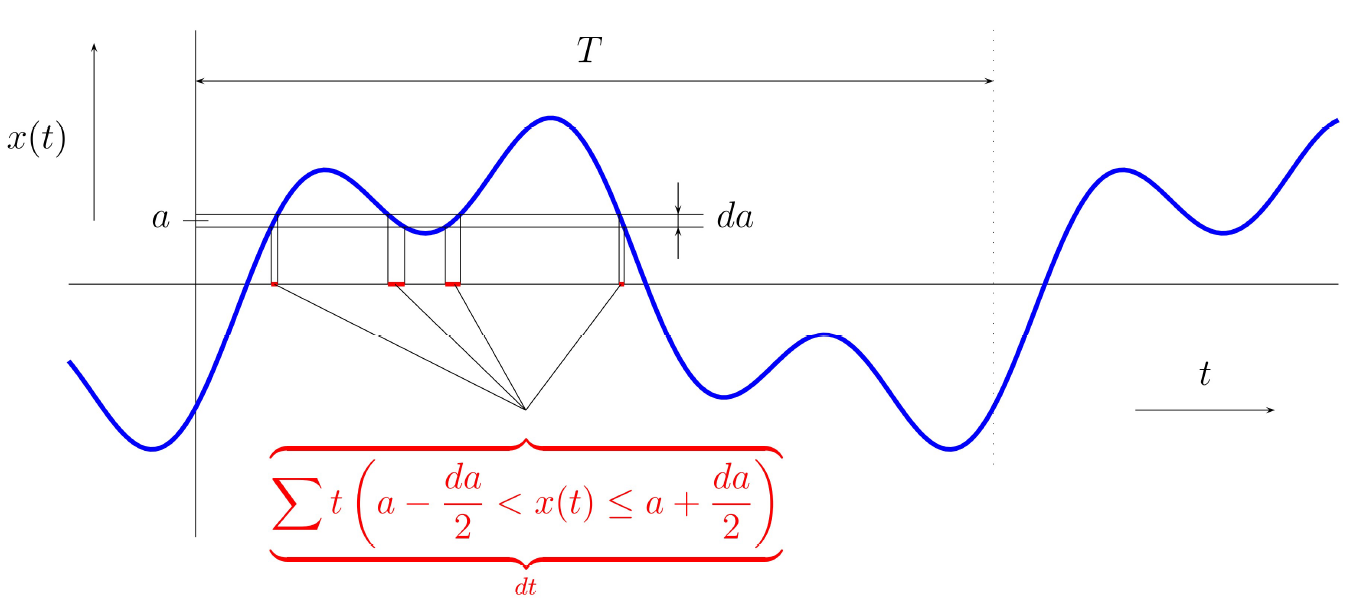
\includegraphics[width=0.75\columnwidth]{images/amplitudendichte.png}
\end{center}


\subsection[Eigeschaften der Amplitudendichte]{Eigeschaften der Amplitudendichte $\bm{p(a)}$}{28}

 \begin{itemize}
    \item  $\int\limits_{- \infty}^{\infty} p(a) \, \diff a = 1 $ \quad (Fläche = 1)
    \item Wahrscheinlichkeit, dass sich Signal in Amplitudenintervall aufhält:\\
        $ P(a_1 < a < a_2) = \int\limits_{a_1}^{a_2} p(a) \, \diff a $
    \item $p(a)$ hat \textbf{keine negativen Werte} 
 \end{itemize}

 \vspace{0.2cm}
\textrightarrow\ Weitere Informationen siehe Anhang Abschnitt ~\ref{Zusammenstellung einiger Dichtefunktionen}


\example{Amplitudendichten}

\textrightarrow\ Siehe Anhang Abschnitt ~\ref{Beispiele - Amplitudendichte}


\subsection{Addition von Amplitudendichten}{34}

Die Addition von zwei \textbf{unabhängigen} Amplitudendichten entspricht einer \textbf{Faltung}
$$ \boxed{ p_a(a) = p_1(a) * p_2(a) = \int\limits_{-\infty}^{\infty} p_1(x_1) \cdot p_2(a-x_1) \, \diff  x_1  } $$


\subsection{Mittelwerte der Amplitudendichte}{29}

\begin{minipage}[t]{0.48\columnwidth}
    \begin{center}
        \myul{\textbf{Linearer Mittelwert $\bm{X_0}$}}
        $$ \boxed{  X_0 = \int\limits_{-\infty}^{\infty} a \cdot p(a) \, \diff a } $$
    \end{center}
\end{minipage}
\hfill
\begin{minipage}[t]{0.48\columnwidth}
    \begin{center}
        \myul{\textbf{Mittelwert $\bm{n}$. Ordnung}}
        $$ \boxed{  X^n = \int\limits_{-\infty}^{\infty} a^n \cdot p(a) \, \diff a } $$
    \end{center}
\end{minipage}


\subsection{Stochastische Signale}{31}

\subsubsection{Gauss-Verteilung, Normalverteilung $\bm{N(\mu, \, \sigma)}$}

\begin{center}
    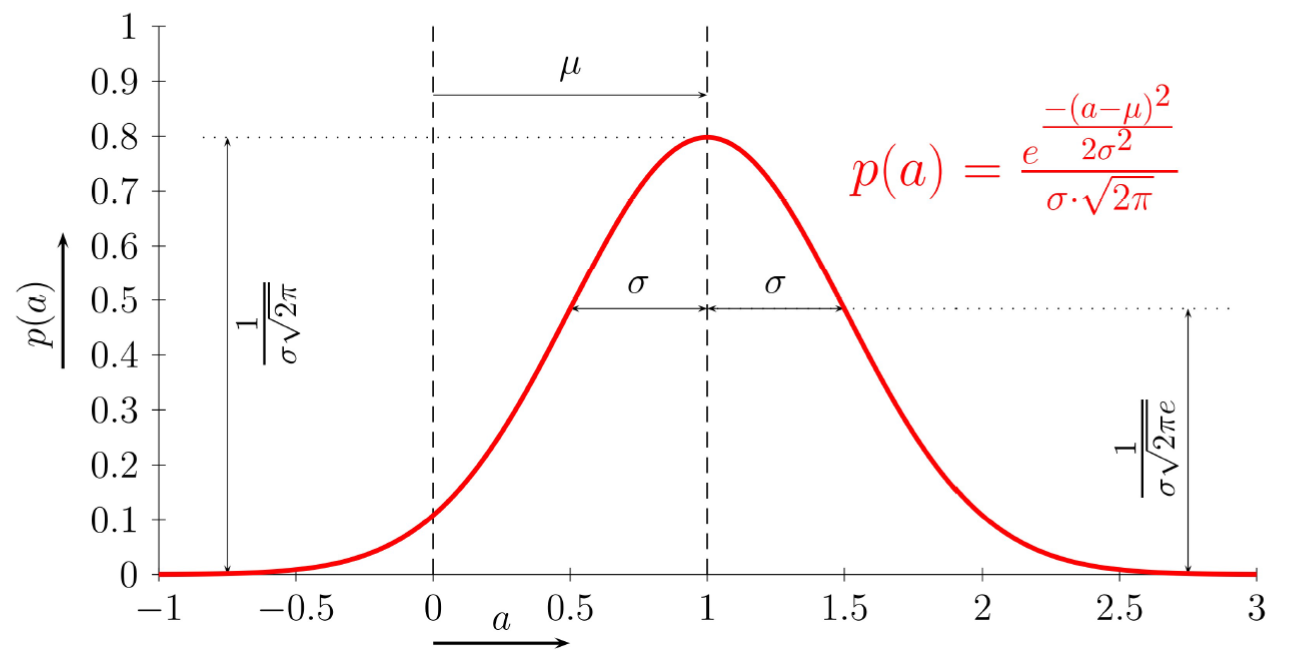
\includegraphics[width=0.8\columnwidth]{images/gaussnormalverteilung.png}
\end{center}
$$ \boxed{p(a) = N(\mu, \, \sigma) = \frac{1}{\sigma \sqrt{2 \pi}} e^{\frac{-(a -\mu)^2}{2 \sigma^2} } } $$

\vspace{0.2cm}
\textbf{Hinweis:} Werden zwei Normalverteilungen miteinander \textbf{gefaltet}, so ergibt sich wieder eine Normalverteilung:

$$ \boxed{ N(\mu_1, \, \sigma_1) * N(\mu_2, \,  \sigma_2) = 
    N \left( \underbrace{ \mu_1 + \mu_2}_{\substack{\mu}} , \, \underbrace{ \sqrt{\sigma_1^2 + \sigma_2^2} }_{\substack{\sigma}} \right) } $$


\subsubsection{Gleichverteilung}{33}

Konstante Amplitudendichte $p(a)$ in einem begrenzen Amplitudenintervall \\
\textrightarrow\ Siehe Beispiel 'Dreieck' im Anhang Abschnitt ~\ref{Rechteck} 

\columnbreak

